\documentclass{article}

\usepackage{array}
\usepackage{amsmath}
\usepackage{amssymb}
\usepackage{graphicx}
\usepackage{subfigure}
\usepackage{color}
\usepackage{undertilde}
\usepackage[colorlinks = true, filecolor = red, urlcolor = blue, linkcolor = black]{hyperref}
\usepackage{pdflscape}
\usepackage{pifont}
%\usepackage{fullpage}
\setlength\textwidth{6in}
\setlength\textheight{8in}
\setlength\oddsidemargin{0.25in} % LaTeX adds a default 1in to this!
\setlength\evensidemargin{0.25in}
\setlength\topmargin{-0.0in} % LaTeX adds a default 1in to this!
\setlength\headsep{0in}
\setlength\headheight{0in}
\setlength\footskip{1in}

\renewcommand{\topfraction}{0.85}
\renewcommand{\textfraction}{0.1}
\renewcommand{\floatpagefraction}{0.75}

\newcommand{\vect}[1]{\ensuremath\boldsymbol{#1}}
\newcommand{\tensor}[1]{\underline{\vect{#1}}}
\newcommand{\del}{\triangle}
\newcommand{\grad}{\nabla}
\renewcommand{\div}{\grad \cdot}
\newcommand{\ip}[1]{\left\langle #1 \right\rangle}
\newcommand{\eip}[1]{a\left( #1 \right)}
\newcommand{\pd}[2]{\frac{\partial#1}{\partial#2}}
\newcommand{\pdd}[2]{\frac{\partial^2#1}{\partial#2^2}}
\newcommand{\nor}[1]{\left\| #1 \right\|}

\newcommand{\circone}{\ding{192}}
\newcommand{\circtwo}{\ding{193}}
\newcommand{\circthree}{\ding{194}}
\newcommand{\circfour}{\ding{195}}
\newcommand{\circfive}{\ding{196}}

\newcommand{\Reyn}{\rm Re}
\newcommand{\Gh}{\Gamma_h}
\newcommand{\Oh}{\Omega_h}
\newcommand{\LRa}[1]{\left\langle #1 \right\rangle}
\newcommand{\LRs}[1]{\left[ #1 \right]}
\newcommand{\jump}[1] {\ensuremath{\LRs{\![#1]\!}}}


\def\arr#1#2#3#4{\left[
\begin{array}{cc}
#1 & #2\\
#3 & #4\\
\end{array}
\right]}
\def\vecttwo#1#2{\left[
\begin{array}{c}
#1\\
#2\\
\end{array}
\right]}
\def\vectthree#1#2#3{\left[
\begin{array}{c}
#1\\
#2\\
#3\\
\end{array}
\right]}
\def\vectfour#1#2#3#4{\left[
\begin{array}{c}
#1\\
#2\\
#3\\
#4\\
\end{array}
\right]}
\date{}
\author{Jesse Chan}
\title{Proposal outline/notes}

\begin{document}

\section{Introduction}

\subsection{Motivation and goal}

\begin{itemize}
\item Adaptivity and stability for CFD problems are issues - cite David Young.
\item To develop a stable $hp$-adaptive scheme for the steady laminar Navier-Stokes equations in transonic/supersonic regimes.
\end{itemize}

\subsection{Literature review}
\begin{enumerate}
\item Finite difference, finite volumes
\item Finite elements

\begin{itemize}
\item Taylor-Galerkin, SUPG
\item Upwind DG, HDG (stabilization?)
\item DPG
\end{itemize}

\item Optimization/NL solvers (?)
\end{enumerate}

\section{Range of CFD problems}

\begin{figure}[!h]
\centering
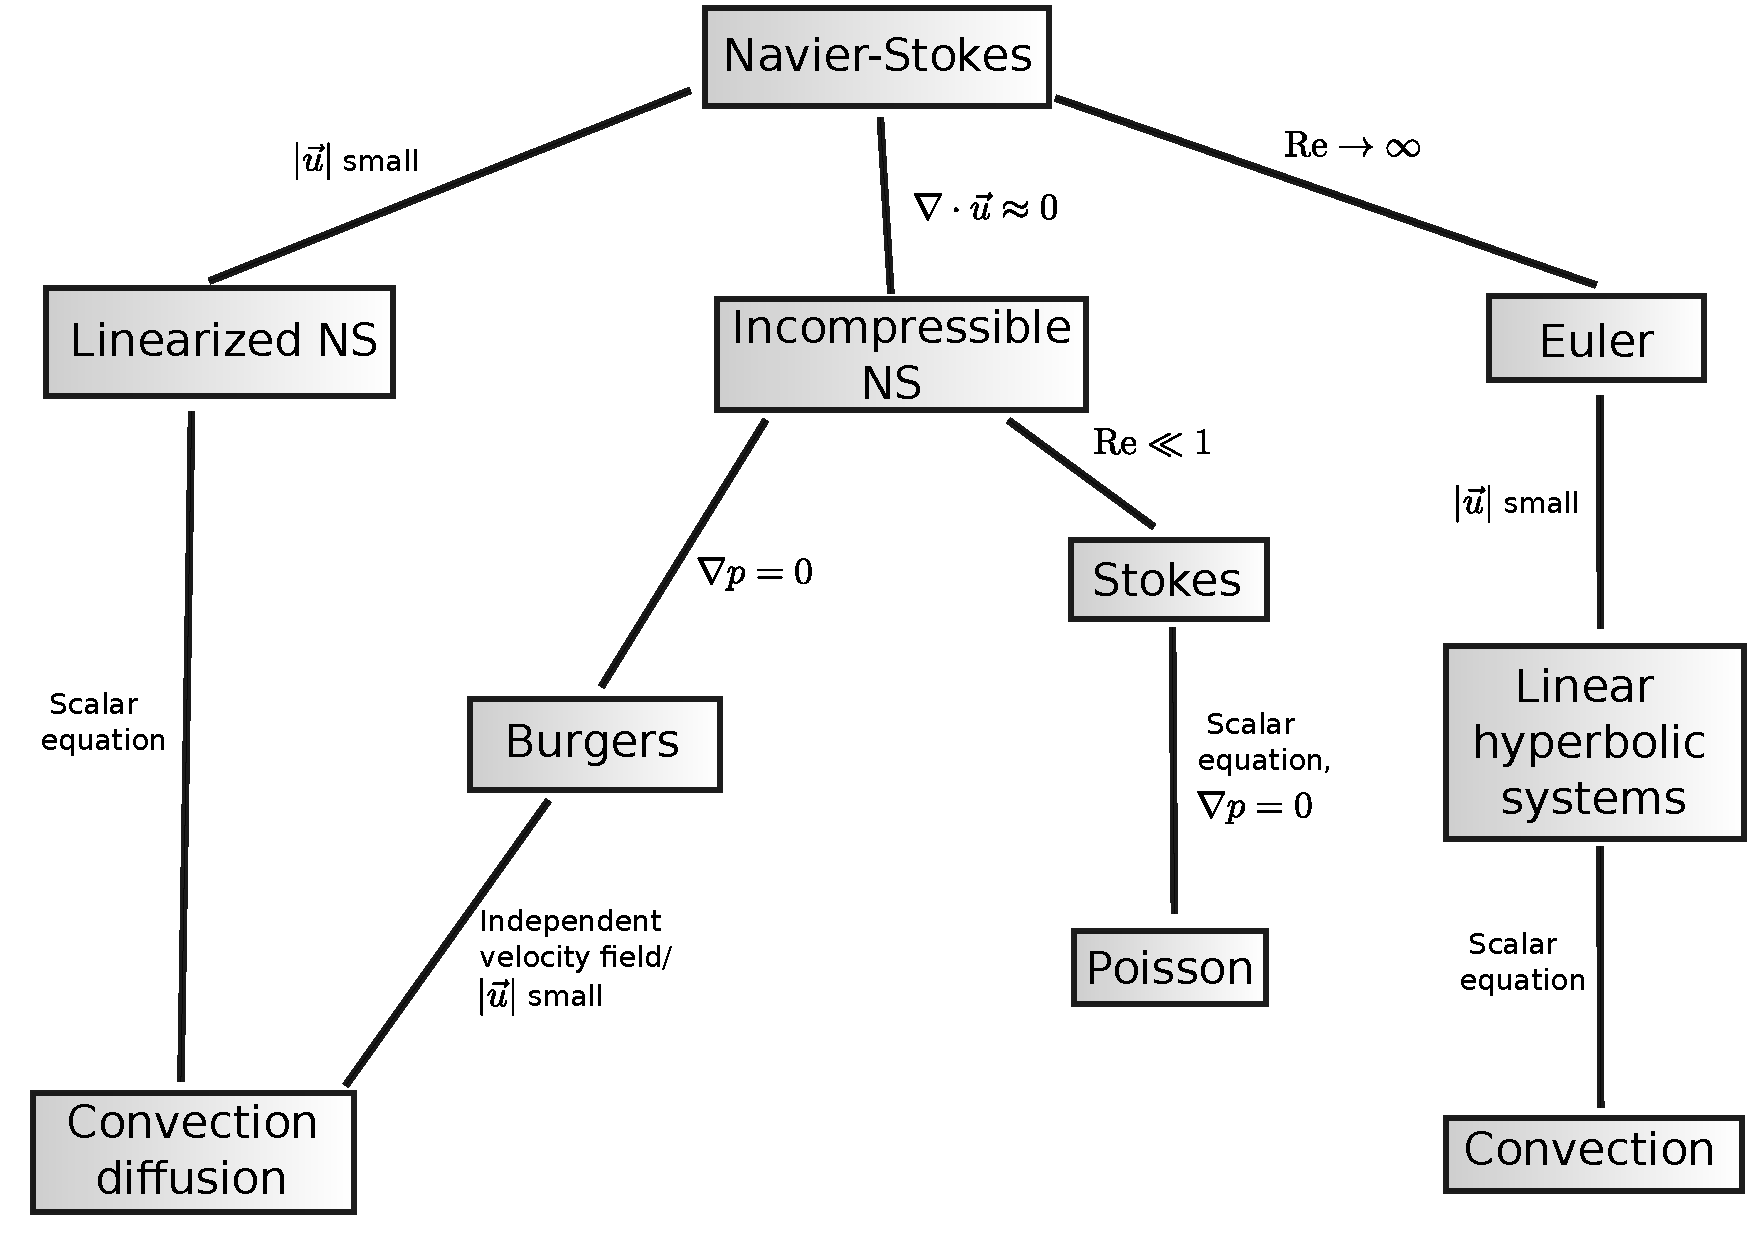
\includegraphics[scale=.4]{CFD_tree.pdf}
\caption{Common CFD problems and their simplifying assumptions.}
\end{figure}

\section{DPG: a minimum residual method for linear problems}



\section{Robustness for convection-dominated diffusion}

\section{DPG for nonlinear problems}

Introduce nonlinear residual to measure convergence, DPG formulation for nonlinear problems. Discuss solution strategies (pseudo-timestep/damped Newton). 

Formulate DPG for Burgers' equation as an example, showing results, then show Navier-Stokes at a broad level. 

\section{Proposed work}

\subsection{Area A}

Analysis of (incompletely parabolic?) convection-diffusion systems

\subsection{Area B}

Nonlinear DPG - Hessian adjoint trick, anisotropic refinements, $hp$-adaptivity, distributed static condensation (if it's not implemented by then). 

\subsection{Area C}

Ramp, bump, airfoil, Euler with NS regularization?

\bibliographystyle{plain}
\bibliography{paper,NS}

\end{document}
